For evaluation purposes, we have used HDF5's \textit{h5perf} performance tool~\cite{h5perf}. h5perf is a tool for testing the performance of PHDF5. It allows configuring various parameters, such as the number of processes to run the test with, number of datasets to be created in the file, amount of data contributed by each process per dataset, amount of data read/written by a process in a single I/O call (transfer size) etc. For our measurements, we created 10 datasets in the file, and the total file size was 64 GB or more.

All tests were performed on the Lustre parallel file system~\cite{lustre} on the Atlas cluster at University of Dresden. The file system has 12 OSTs with a stripe size of 1 MB. The file system is connected to the compute nodes using an SDR Infiniband link. 
The cluster has 92 nodes with 64 cores each and 64 to 512 GB memory. All nodes are AMD Opteron 6274 running at 2.2 GHz.

Our tests were configured such that we spawn a maximum of 4 processes per node. Tests run with less than 4 processes utilized a single node. 

%\begin{figure}[!t]
%\centering
%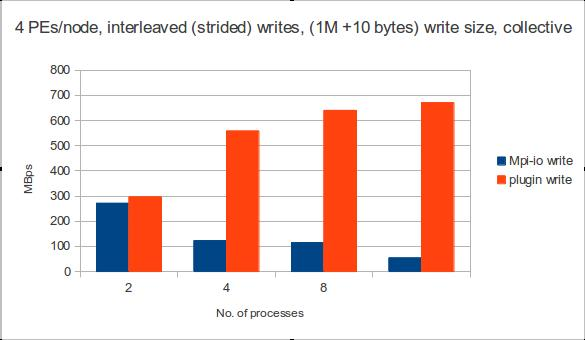
\includegraphics[width=2.5in]{4pes_interleaved_1m10_coll_writes}
%\caption{A sample HDF5 file}
%\label{writes}
%\end{figure}
%
%\begin{figure}[!t]
%\centering
%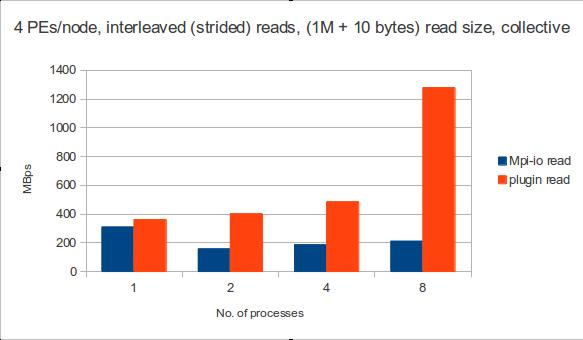
\includegraphics[width=2.5in]{4pes_interleaved_1m10_coll_reads}
%\caption{A sample HDF5 file}
%\label{reads}
%\end{figure}


